\section{Design}
The main design components are 1) Introspection, 2) Visualization, 3) Data Analysis and, 4) Provenance. The main goal is to detect  anomalies in an application behavior during runtime.

\begin{figure}[th!]
 \centering
  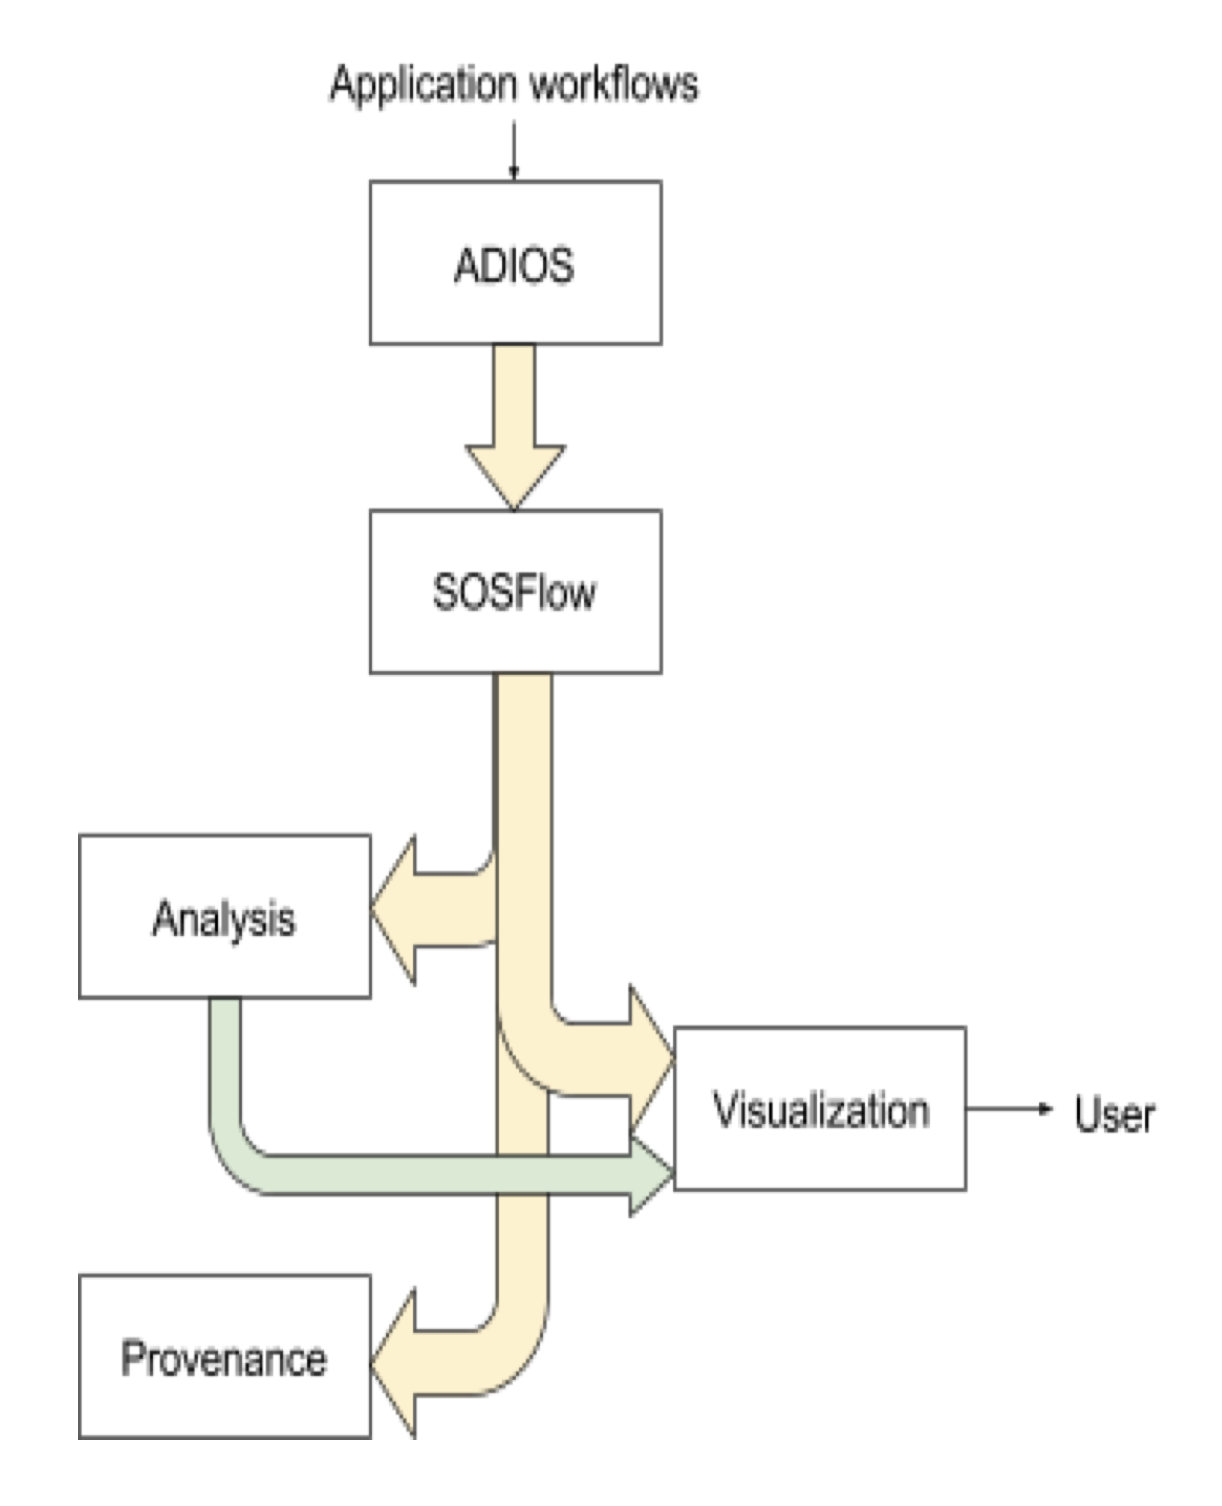
\includegraphics[width=0.4\textwidth]{Figs/design_Y2}
 \caption{Chimbuko information pipeline.}
\label{designfig:1}     
 \end{figure}


\subsection{Introspection ( TAU + SOSFlow)}
The University of Oregon (UO) will provide the CODAR project with infrastructure to make performance data accessible online (i.e., performance monitoring) in a form that permits in situ analysis and reduction. In the first year, a performance monitoring prototype will be created for demonstration of online access using three milestones. Subsequent years (as necessary) will see hardening, testing, tuning, and deployment of tools with relevant CODAR applications.  Configurability is a key concern in this effort, allowing for targeted and multi-resolution access to data.
\begin{enumerate}
\item Extensible Monitoring Plugin Support: TAU will be extended to provide a plugin framework where an event stream will be exported by each MPI rank. An analysis plugin will subscribe to events such as initialization/finalization, metadata values, interval event timers, and counters.  The TAU team will modify the current hardwired SOS integration to be a plugin. The SOS client plugin will monitor the data stream at runtime, and provide aggregation/filtering/reduction utilities.  The SOS client plugin will also provide a feedback path to TAU, in order to increase/decrease resolution of measurement (sampling rate, callpath depth, hardware counters, etc) if/when that capability is added to TAU.
\item Online Monitoring Access: Profile, event trace and metadata events will be provided to the analysis through SOS\cite{Chad}. In a coupled application / workflow scenario, SOS will regularly/periodically aggregate TAU data over the SOSflow infrastructure.  This data will be extracted from SOS through an SOS analysis extension that will output the aggregated event stream as ADIOS streaming output.  The SOS extraction client will have the ability to filter data from one or more specific nodes, rather than just an aggregated data stream.  The CODAR team will use the ADIOS stream for supporting their trace analysis tools and anomaly detection. These tools may be shipped with TAU as contributed software.
\end{enumerate}

\subsection{Required Data and the Stream Interface}
\label{subsection:features}
Figure~\ref{designfig:1} gives the Chimbuko pipeline for information. The figure shows how performance data streams through Chimbuko's modules. For data analysis and visualization module, the following features are to be collected from SOSFlow:
\begin{enumerate}
\item {For each component in a workflow:}
\begin{enumerate}
\item start and end timestamp
\item call stack
\item memory allocation
\item IO in network or disk
\item total Communication time
\item effective  communication time
\item effective computation time
\item idle time
\item number of synchronization points/ barriers
\item communication size
\item communication between functions
\item communication between nodes
\end{enumerate}
\item  For each workflow:
\begin{enumerate}
\item number of components
\item amount of communication for each pair of components
\item effective communication for each pair of components
\item communication size for each pair of components
\item aggregated number of communication calls 
\item aggregated communication execution time
\end{enumerate}
\end{enumerate}

For visualization module, we also require the outlier results from analysis module in terms of the array of call ID, MPI execution ID, or workflow ID. 


\subsection{Data Analysis}
In this year we aim to provide online performance analysis. Last year, we prototyped off-line performance anomaly detection by using Local Outlier Factor (LOF) algorithm. In order to push our data analysis to online level with strong scalability, we plan to design or evaluate online anomaly detection algorithm  with the features, given in Section~\ref{subsection:features}, to be collected from SOSFlow.

\subsubsection{Interface design between online data analysis and SOSFlow}
The online data analysis could be implemented as two styles. (1) Consumer-Producer where SOSFlow will be the performance profile/trace stream producer, and our online analysis will be the consumer implemented as its client. (2) Another design choice is that we may consider our performance analysis module as a plug-in within SOSFlow and get performance data stream locally.
\subsection{Performance Visualization}
Last year, we finished off-line performance visualization focusing on ``overview first, details on demand'' scheme. For this year, analysis before visualization is mandatory to enable real-time data consumption. We thus aim to provide online performance visualization coupled with performance analysis of the chimbuko team.

Therefore, in order to establish the connection between the analysis module, SOSFlow, and the user, the mission of visualization module has two folds: first, a user exploration interface to visualize, monitor and interact with the analysis results and performance data; second, a back end communication to the analysis module and streaming data flow from SOSFlow. 

As deliverables, we will complete the following tasks:
\begin{itemize}
\item A set of visual analytics modules at the front end to convey analysis results and provide interaction
\item Methods on the back end to communicate with data analysis module and SOSFlow. Two styles are considered: (1) passive mode, where SOSFlow or analysis module performs as server, and sending update data to visualization module as its client; (2) active mode, where user queries the detailed information from SOSFlow or analysis module. 
\item Methods on the back end to maintain a local database collecting only the details of the outliers and other necessary information for users to query workflow details.
\end{itemize}

\subsection{Prescriptive provenance for online analysis}
This year we are expecting to extract and store provenance relevant to online performance analysis.  Provenance will be extracted, aggregated, and made available while the simulation is in progress with the TAU/SOSFlow plugin.  As provenance can be very verbose and persisting provenance for an entire run is impractical, we plan on persisting detailed provenance ONLY for the anomaly events or events of interest detected by online performance analysis.  Ultimately, provenance is to be persisted in SOSFlow for a moving window prior to and posterior to an event with the additional capability to increase or decrease the verbosity of provenance (size and granularity of the moving window) selected for storage around the event.  In addition, static information describing the system, runtime configuration, and  workflow or application metadata similar to what is already extracted for offline will be persisted at the on start and end of the run (static information).  This is what we call prescriptive provenance: provenance selection and use prescribed by the results of performance data analysis described above.  Persisted prescriptive provenance is an end-product of the analysis after training sets have been built.
Specifications of the moving window of provenance prior to an outlier event will need to be studied for tradeoffs.  For instance, we will study if this window is defined in terms of execution time or number of timesteps.  Constraints of size will apply, as well as tradeoffs in the amount of details needed, and will need to be balanced with usefulness to a scientific code developer.
The metadata values that need to be extracted for prescriptive provenance will vary depending on the application and the node architecture where application components run.  Features given in Section~\ref{subsection:features} are of great interest, with a priority first given to detailed communication, understood as mpi communication, then I/O.  The choice of communication as a priority for data extraction is motivated by its demonstrated impact on performance in 2017 for applications such NWChem and LAMMPS. 